\chapter{Literature Study}

The literature study includes current knowledge about the subect, is evaluated, and consists of fundamental concepts to note.\\

Infrared light extends from the nominal red edge of the visible spectrum at 700 nanometers (430 THz) to 1 mm (300 GHz) \cite{ir_wiki}. The infrared light to be used for NDVI analysis is between 700 and 1000 nm due to silicon response \cite{ir_wiki}, and is known as near infrared light (NIR).

\begin{figure}[H]
\centering
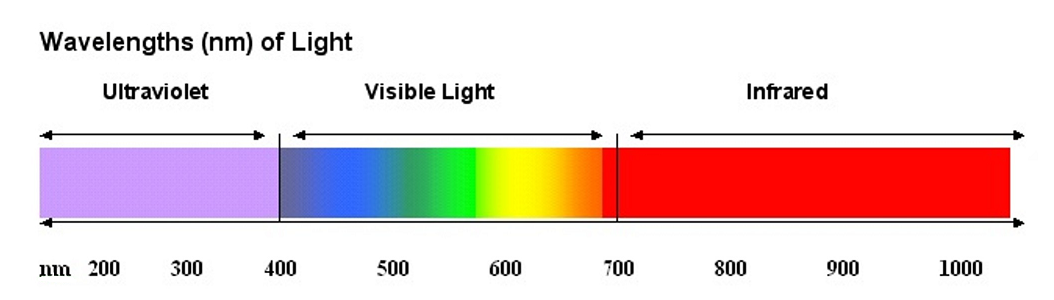
\includegraphics[scale=0.35]{images/ir_spectrum.png}
\caption{Wavelengths of light \cite{ir_spectrum}}
\label{fig:ir_spectrum}
\end{figure}

The normalized difference vegetation index (NDVI), which forms the base of this project, is a simple graphical indicator that can be used to analyze remote sensing measurements, typically but not necessarily from a space platform\footnote{Aerial footage will always be higher resolution, with each pixel capturing $cm^2$ as opposed to $m^2$}, and assess whether the target being observed contains live green vegetation or not\cite{ndvi_wiki} as in Figure \ref{fig:ndvi_british}.

\begin{figure}[H]
\begin{subfigure}{0.5\textwidth}
\centering
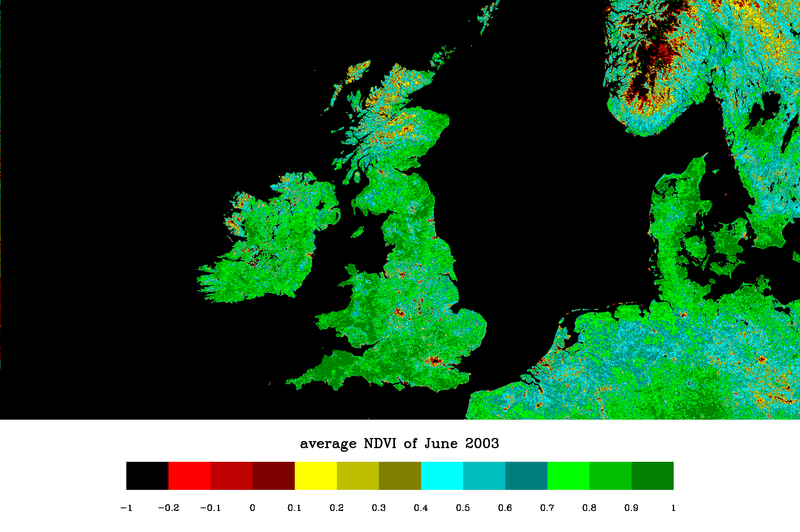
\includegraphics[scale=0.25]{images/NDVI_062003.png}
\caption{June 2003}
\end{subfigure}
\begin{subfigure}{0.5\textwidth}
\centering
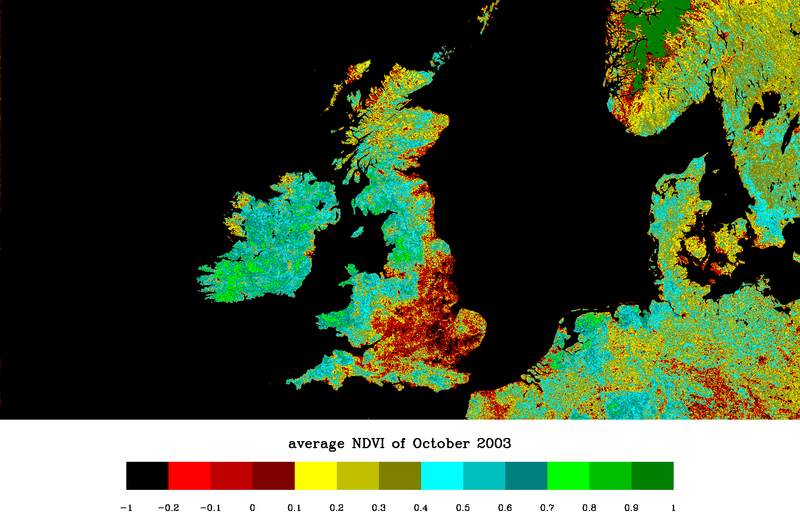
\includegraphics[scale=0.25]{images/NDVI_102003.png}
\caption{October 2003}
\end{subfigure}
\caption{Average NDVI over the British Isles \cite{ndvi_wiki}}
\label{fig:ndvi_british}
\end{figure}

The NDVI is calculated using the following formula for each pixel:\\

\begin{equation}\label{eq:ndvi}
{\displaystyle{\mbox{NDVI}}={\frac {({\mbox{NIR}}-{\mbox{Red}})}{({\mbox{NIR}}+{\mbox{Red}})}}}, \in [-1.0, 1.0]
\end{equation}

where red and NIR stand for the spectral reflectance measurements acquired in the red (visible) and near-infrared regions, respectively.

\begin{figure}[H]
\centering
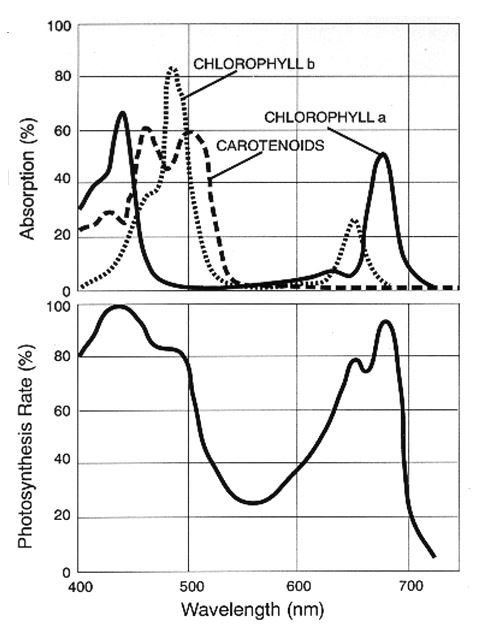
\includegraphics[scale=0.5]{images/chlorophyll.jpg}
\centering
\caption{PAR and absorption spectrum \cite{ndvi_wiki}}
\label{fig:chlorophyll}
\end{figure}

In Figure \ref{fig:chlorophyll}, typical photosynthetic action in the photosynthetically active radiation (PAR) spectral region for live green plants is shown, beside absorption spectra for chlorophyll and carotenoids. Solar radiation is absorbed within this region as a source of energy. \\

Leaf cells re-emit solar radiation in the near-infrared region because the photon energy at wavelengths longer than 700 nm is not large enough to synthesize organic molecules, even though it comprises approximately half of the total incoming solar energy. If it were absorbed, it would only result in damage and overheating of the plant.\\

The NDVI is similar to a mere ratio of infrared light to visible light, yet since it is not normalised, one can have infinite values.\\

The rationale behind the NDVI is that one can exploit the strong differences in plant reflectance to determine their spatial distribution.\\

NDVIs have been around for many years. 

Satellites

That company in CT.


Since the proliferation of UAVs, there has been an increased effort to find more cost effective solutions to commercial applications, not excluding NDVI analysis.
There has been much action in recent years 